\subsection{Communications (COMM)}
Due to the fact that the main objective of the mission is to provide internet
communications along the globe, this subsystem is considered critical for the
mission success. The communications subsystem (COMM) will be the one in charge
of providing effective transmission and reception of the radio signals between the
satellite and both the ground stations and other satellites, within \MissionName
constellation or third part satellites.

\subsubsection{Design process}
In order to design the communications subsystem, we have to identify which are
the communication needs of our satellites. That needs can be categorized in two types:

\begin{itemize}
	\item \textbf{Ground communications}. That are communications between the
	satellite itself with ground systems, both fixed ground stations (GS) and
	smaller, portable, IoT devices.
	\item \textbf{Inter-satellite communications}. Which are communication
	with other satellites in orbit, within our constellation or not.
\end{itemize}

This two needs sets a first requirement for the communications subsystem:
the antenna system shall be separated in two independent antennas, one for the
ground communications (in the following, called Earth-antenna) and another one for
the inter-satellite communications (called space-antenna). This approach as also the
advantage of some kind of redundancy; in case of failure of the Earth-antenna, the
satellite could still be operative as a inter-satellite link.

The two sets of antennas are two different devices and may have different
specifications, base frequency, transmission/reception patterns...

\paragraph{Earth-antenna}

The band frequency in what the Earth antenna would work
is restricted by the Earth-atmosphere blocking frequencies, that are shown in
figure \ref{fig:frequency_atmosphere_opacity}, so in the practice they are limited
to the radio frequency range from around 2 cm wavelength (15Ghz) to 20m (15MHz).

\begin{figure}[h]
	\centering
	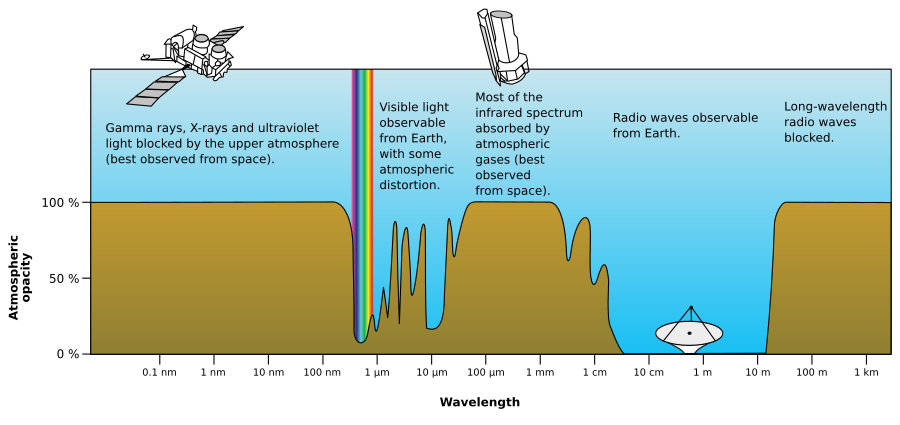
\includegraphics[width=\textwidth]{img/earth_freq.png}
	\caption{Atmospheric electromagnetic radiation opacity}
	\label{fig:frequency_atmosphere_opacity}
\end{figure}

The chosen frequency shall be in the range of few gigahertz, because lower
frequencies in the range of megahertz won't give us enough bandwidth to send and
receive internet data; and higher frequencies use more complex antennae.

For the Earth antenna there were initially two main architectures. One of them
is to use a parabolic antenna that exists in the current cubesat state-of-art.
The main problem with this antennas is that the bean shape is quite narrow and
it would only cover a small portion of the Earth surface.

Another approach very simple and cheap is to use a deployable helicoidal antenna.
Which consist in some wires arranged in helicoidal way, that deploy by themselves
when activated. There exists in the market some products that are tested to work
fine and they are prepared for cubesat dimensions and mass requirements.
